\chapter{Parallel Impulse Solver}\label{cha:impl}

\section{Spherical Decomposition}
\cite{gpugems} presents a method for collision detection and response using spherical
decomposition. By subdividing the geometry into a collection of spheres one get an
approximation of the shape. Since each new geometry is locally convex collision
detection is much simplified, but the global result of the decomposition still have
concave properties. Since each new geometry is the same primitive only
one type of collision detection and response is needed. For an example of geometries
decomposed in this manner see figure~\ref{fig:bunnies}.

\begin{figure}[H]
  \centering
  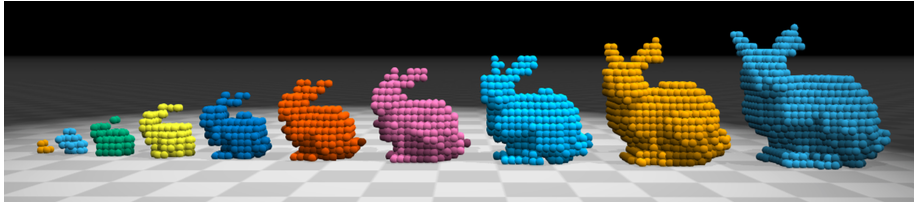
\includegraphics[width = 0.9\textwidth]{flexBunnies.png}
  \caption{Varying degrees of spherical decomposition of the Stanford bunny.
  Image collected from the flex paper by~\cite{flex}}
  \label{fig:bunnies}
\end{figure}

\section{Multiple contacts in sequential solvers}
When solving with multiple contacts between a body pair one can rewind time to
find the first collision
that occurred in the system (a single body pair, or globally), process it first
then step forward until the next collision and so forth. However this method can
be quite time consuming and lack parallelism since we get an ordering in the solver.
If we do not back the system in time and
instead simply solve all collisions we have currently and take some special care
towards interpenetration we would end up with incorrect physics. The problem
becomes quite apparent through the following example.
In figure~\ref{fig:ballsExpected} we see the expected result and in
figure~\ref{fig:noSplit} we see the result if one uses a naive implementation of
parallel impulses.

\begin{figure}[H]
  \centering
  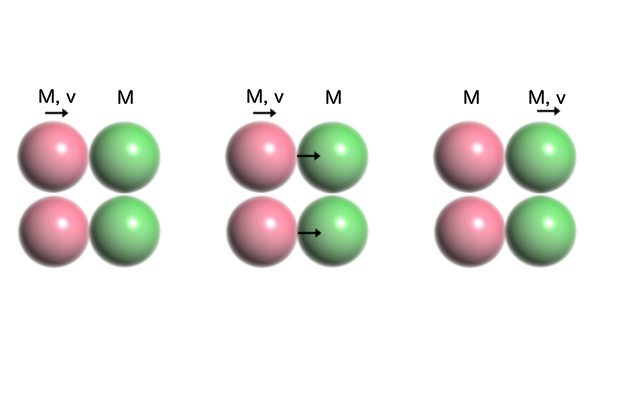
\includegraphics[width = 0.8\textwidth]{ballsExpected.png}
  \caption{The expected result of the collision between the rigid body consisting
  of the red balls and the rigid body consisting of the green balls.}
  \label{fig:ballsExpected}
\end{figure}

\begin{figure}[H]
  \centering
  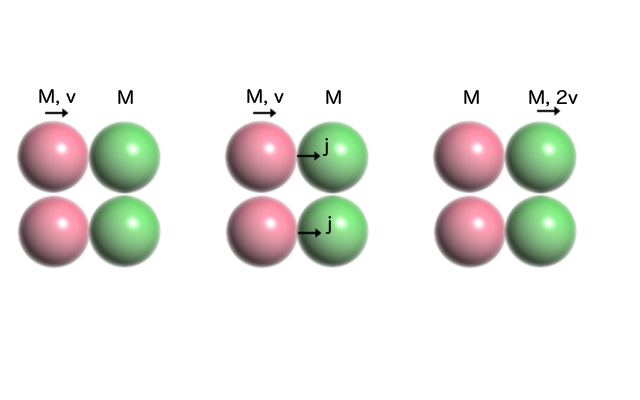
\includegraphics[width = 0.8\textwidth]{ballsNoMassSplit.png}
  \caption{Calculating all impulses in parallel can lead to too high end velocities.}
  \label{fig:noSplit}
\end{figure}

This problem can be remedied by only solving one impulse between a body pair at a time.
This can be achieved as above stated by either backing up time until there
is only one collision, or a few collisions and then solve one of them, chosen
arbitrarily. This gives rise to a order dependent system, and is something which
makes for difficult realizations in parallel algorithms. Another approach popularized
by Erin Catto in his Box2D is 'Sequential Impulses' which solves the worst interpenetration
on each respective body pair, updates the velocities and iterates for a few iterations.
One interesting aspect here is that negative impulses are allowed in intermediate
results. However as the name suggests it is most suitable for a sequential implementation.
Both of the methods above suggests that only one collision between a body pair should
be solved at a time which leads to sequential processing. For more details see \cite{catto}.
This method could arguably be parallelized in the sense that each body could be
processed in parallel, however a different approach is used for this thesis.

\section{Mass splitting}\label{sec:massSplit}
\cite{tonge} describes, in their paper, a parallel constraint based solver
using mass splitting. A similar approach where we split the mass prior to
calculating the impulses by the number of collision between the two bodies. The
calculated impulses are then applied to the original object.

\begin{figure}[H]
  \centering
  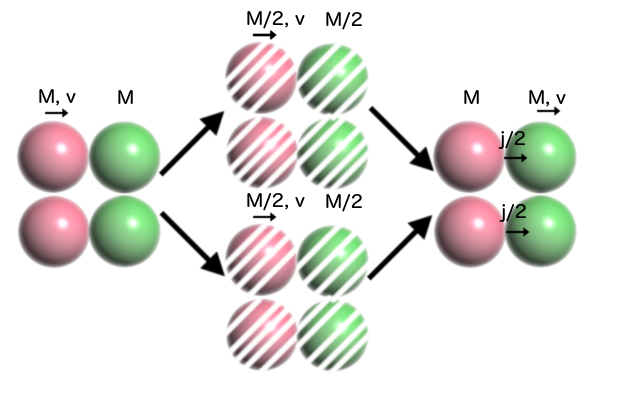
\includegraphics[width = 0.8\textwidth]{ballsMassSplit.png}
  \caption{By mass splitting the objects by the number of interbody collisions
  and applying the resulting impulses to the non-split object we get the expected result.}
  \label{fig:massSplit}
\end{figure}

For this method to be implementable we need to count the number of collisions between
every body pair. This is described in further detail on page~\pageref{sec:colMatrix}.

With $\vec{j}$ defined as in equation~\ref{eq:finalJ} one would simply divide $\vec{j}$ by
the number of collisions between the collision pair, here defined as $k$. The final modification to
$\vec{j}$, before applying it to the bodies then becomes the following.

\begin{equation}
  \vec{j}_{mass split} = \frac{\vec{j}}{k}
\end{equation}

\section{Collision matrix}\label{sec:colMatrix}
As previously mentioned in section~\ref{sec:massSplit} we need to count the collisions
between all collision pairs to acquire correct impulses. A decent way to perform
this is to keep a matrix $C$ keeping count of all collisions. $C_{i,j}$ would
contain the number of collision between body i and body j. This matrix would be
zero throughout the diagonal and symmetric. $C_{i,j} = C_{j,i}$ would of course
be satisfied and technically more data than required is allocated by letting $C$
be an M-by-M matrix where only M/2-M elements are required (where M is the
number of bodies). This reduction in size
has not been implemented, and instead the full M-by-M matrix is used.

A reasonable location in the shader stages for adding the collisions are during
the collision detection shader, each detected collision increments $C_{i,j}$
 through an atomic increment. A drawback of the atomic
 operations are that they may affect the performance of shaders negatively. In
 other words, the benefit that an algorithm comes with have to outweigh the potentially
 slow atomic operations.

\section{Collision Detection}
Initially a brute force collision detection was tested. With $O(n^2)$ it was too
slow and had poor scaling as expected. ~\cite{gpugems} suggests spatial partitioning
by ways of a uniform grid for collision detection. This method is especially suitable
for the spherical decomposition since for fixed sphere radius we can select an optimized
grid size. In addition both~\cite{gpugems} and~\cite{fastnearest} claim that sorting
the collisions by bin number increases memory coherence and overall performance.

Each cell in the grid is $d x d x d$ where $d$ is the diameter of the largest sphere
present in the system. The grid represents 3D space and for simplicity the grid is
implemented as being $mxmxm$.

\subsection{Grid construction}
When using the sorting version of the grid construction, initially we need to count
the number of spheres in each bin and then create the exclusive prefix sum for the sorting
step. The exclusive prefix sum is calculated on the GPU as described in GPUGems chapter 39.
With the exclusive prefix sum at hand we can reset the bin counters and start the sorting.
For each sphere calculate which bin it belongs to, at the bin index check the prefix sum,
use the prefix sum as index for ordering the particles. The pseudocode below describe
the process.

\begin{algorithm}[H]
  \begin{algorithmic}[1]
  \State binIndex = hashFunc(pos);
  \State gInd = thisGlobalThreadIndex;
  \State index = prefixSum[binIndex] + atomicAdd(binCount[gInd],1);
  \State outPutSpheres[index] = inputSpheres[gInd];
\end{algorithmic}
\end{algorithm}

The hash function used for this thesis is a simple flooring of the x,y,z coordinates, a
division by the cell size ($d$) and an offset to let us center the grid over our wished domain.
\begin{equation}
  \vec{id} = floor((\vec{p}-\vec{offset})/d)
\end{equation}
Accessing the correct bin, given m bins per dimension and $\vec{id} = [idx,idy,idz]$, becomes:
\begin{equation}
  binIndex = idx + idy*m + idz*m^2
\end{equation}

The prefix sum ensures we know beforehand how much space (or number of particles)
each bin needs. With the atomic add we can properly index into that subspace of the
array. The two following figures describe the process of sorting through prefix summation.

\begin{figure}[H]
  \centering
  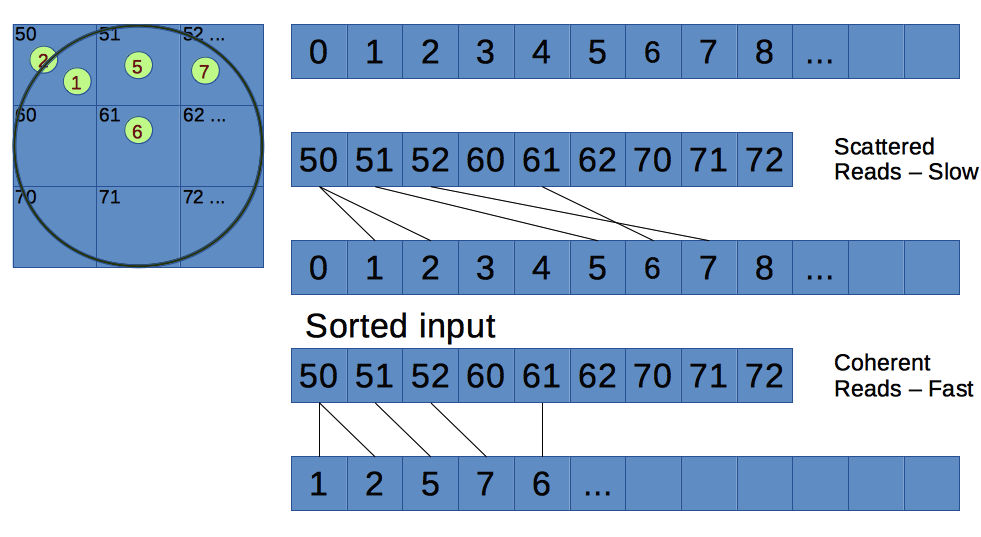
\includegraphics[width = 0.8\textwidth]{prefix1.png}
  \caption{By sorting the spheres we can get more coherent reads.}
\end{figure}

\begin{figure}[H]
  \centering
  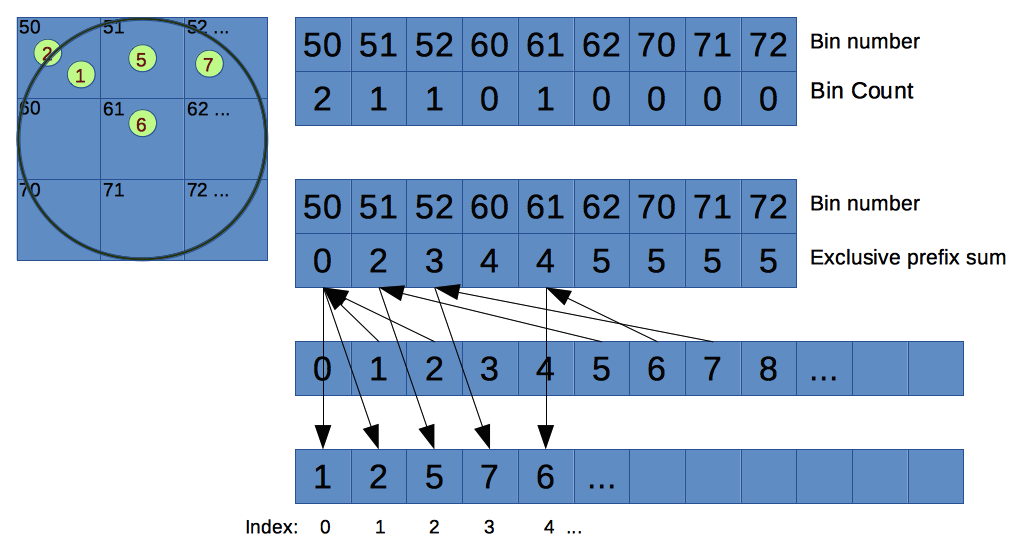
\includegraphics[width = 0.8\textwidth]{prefix2.png}
  \caption{The sorting can be performed through a exclusive prefix sum.}
\end{figure}

The overall flow of the collision detection can be summarized as below.

\begin{algorithm}[H]
  \begin{algorithmic}[1]
  \State gridCounting with atomicAdd
  \State exPrefixSum through reduction
  \State reset gridCount
  \State reorder particles with exPrefixSum and atomicAdd into gridCount to offset.
  \end{algorithmic}
\end{algorithm}

\subsection{Particles outside the grid}
Particles can collide even when outside the grid due to the indexing
being clamped to the grid, see figure~\ref{fig:gridStretch}.

\begin{figure}[H]
  \centering
  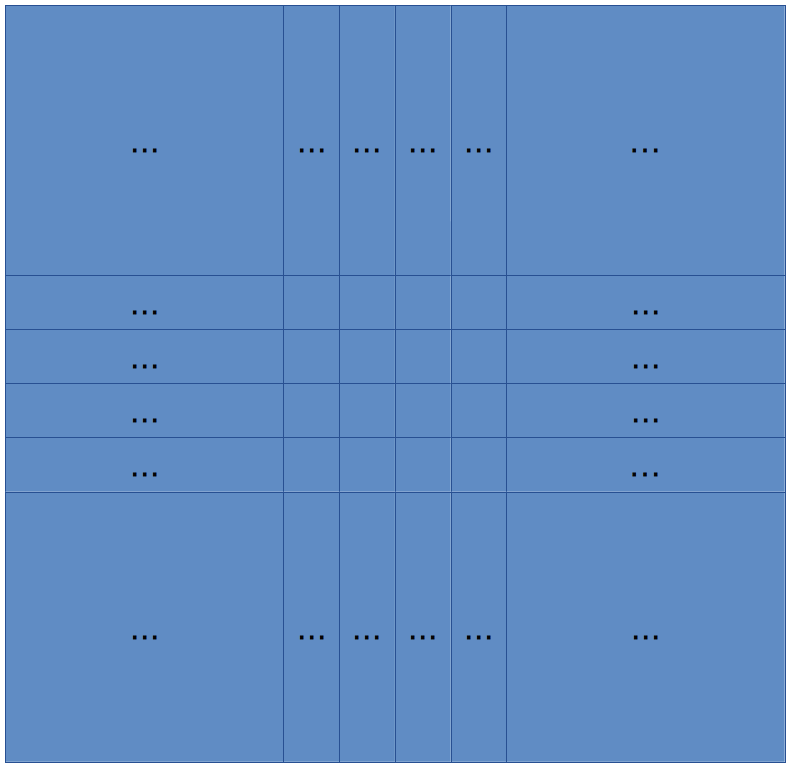
\includegraphics[width = 0.8\textwidth]{gridstretch.png}
  \caption{The cells on the edges extend infinitely due to a clamping.\label{fig:gridStretch}}
\end{figure}

However, the cells at the edges are technically infinite
in size (limited by data types) and can therefore contain a very large amount of particles and the collision
detection step may suffer greatly in performance. Consider the following two situations;
About half of the particles are initially outside the simulation domain; The grid's
cell size is doubled thus moving most of the particles outside into the domain, but
each collision detection will have to search through more particles.
The latter was during testing faster. While each cell became worse, it was better
than letting a few cells execute slower. This is not surprising since this is a
parallel system. In the best case the execution time of the whole system would be
the slowest path in total through the system. This is not however always the case
since not all particles can execute in parallel.

\section{Stabilization iterations} \label{sec:stabil}
The velocity and impulse step are iterated several times to stabilize and solve
interpenetrations by a percentage of the distance as previously described.

The number of iterations need to be high enough for the current situation, below
in the figure is a situation where the number of iterations is too low, with the
number of iterations being 2. When too few iterations are used tunneling can occur
and in some extreme cases the bottom cubes have begun penetrating through the bin.

The spheres are assumed to be in contact however
the figure leaves some space between them for easier reading of the figure.

\begin{figure}[H]
  \centering
  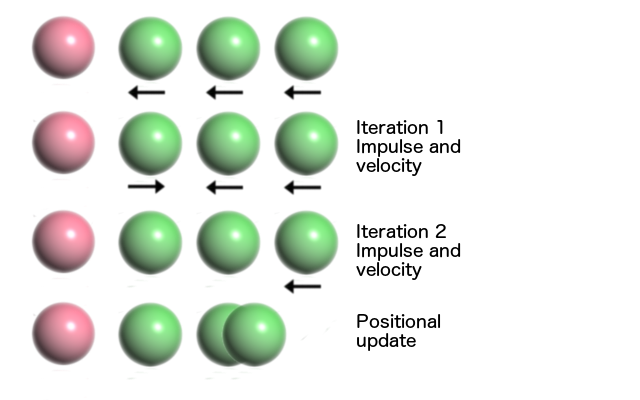
\includegraphics[width = 0.8\textwidth]{nIterationSteps.png}
  \caption{Red sphere is a static object. From top to bottom iterations increase. At the last row the positional update is visualized where interpenetration happens due to too few iterations.}
  \label{fig:flow}
\end{figure}

Unfortunately with higher stacking and increased number of objects in tight proximity,
the number of iterations needed increase or a smaller time step is needed.

\section{Shader structure}
For this implementation OpenGL 4.5 with Compute Shaders are used as the interface
for the GPU. In Compute Shaders you have plenty of tools for workgroup synchronization
but to synchronize globally across different workgroups one split the program into
different shaders and synchronize from the CPU. This is done by ways of barrier bits.Global synchronization
is performed between every shader, i.e. between each box in the flow chart, in the figure~\ref{fig:flow}. Green
boxes in the figure represent shader stages which are dispatched with a thread per
sphere, whereas the blue dispatch across bodies instead.

\begin{figure}[H]
  \centering
  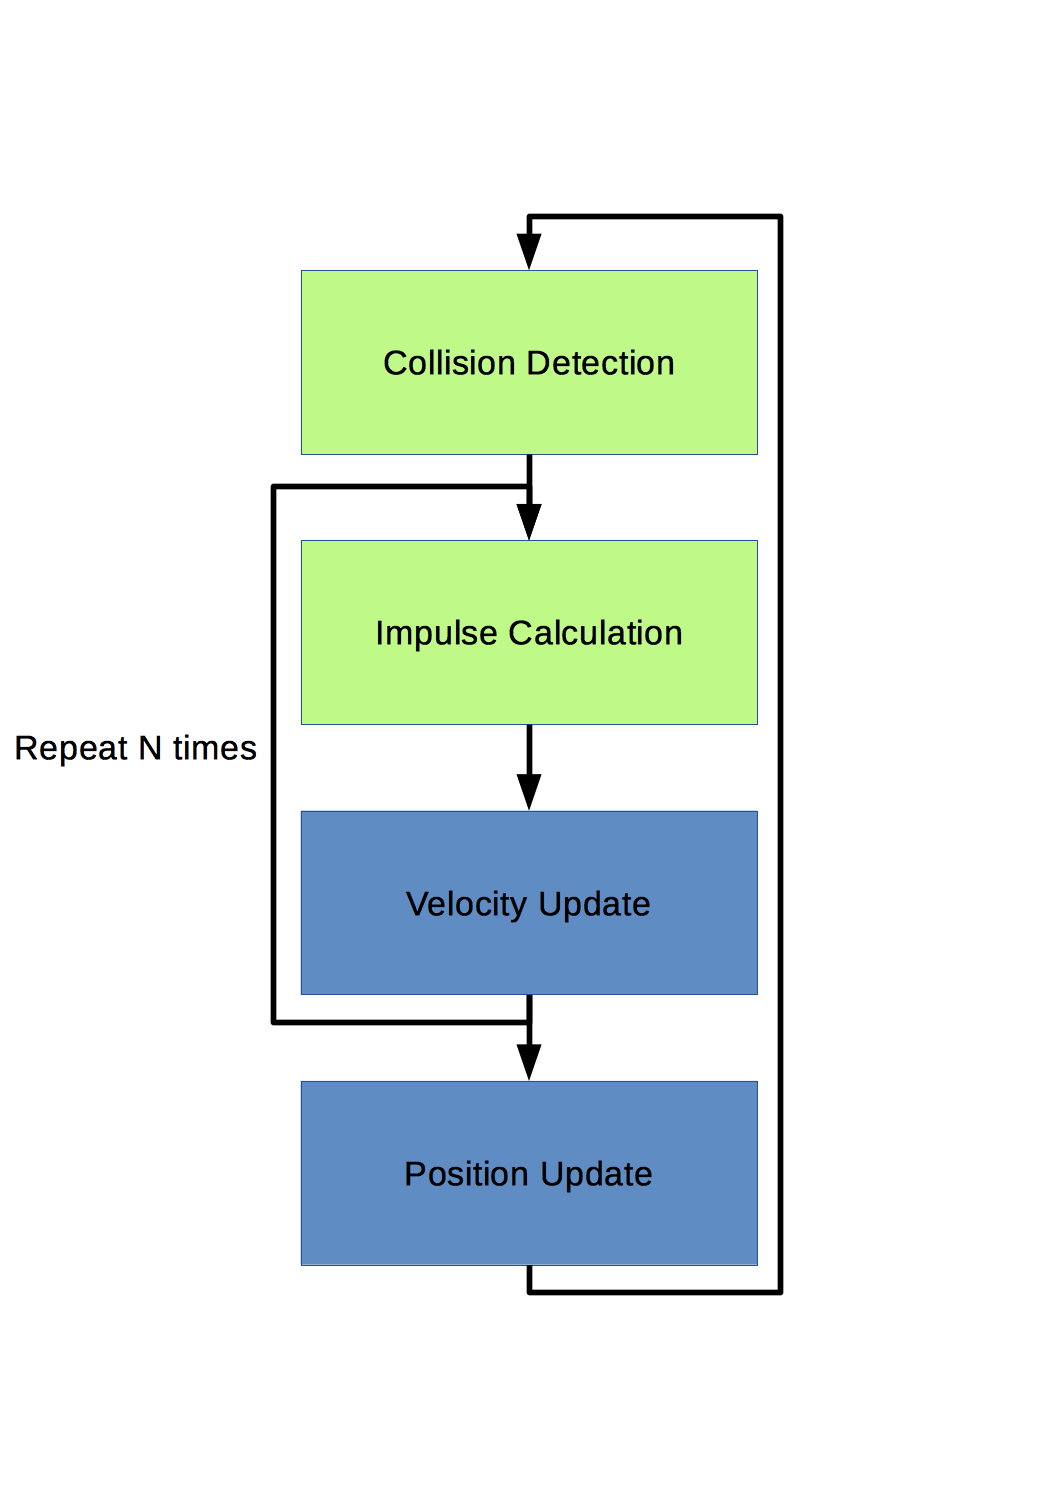
\includegraphics[width = 0.8\textwidth]{shaderflow.png}
  \caption{Flow chart of the different shaders involved. Green shaders are dispatched over spheres and blue over bodies.}
  \label{fig:flow}
\end{figure}


\subsection{Collision Detection}
The collision detection is preformed as mentioned through sorting and spatial partitioning.
The main problems with this approach is the limited domain which can be simulated.
The bins size should for optimal search conditions be exactly the diameter of the largest
particle in the system however larger bins can be used with the penalty that more
particles has to be checked, but it results in a larger valid simulation domain.

When the collision grid and reordering is done one can find the true collisions
among the candidates. All candidates reside in the the 26 surrounding neighboring
grid cells and the particles' own cell. The distances are measured between all
candidates and the true collisions are saved to a collision manifold, a structure
containing the id of the particle, for this implementation a finite number of
contacts can be assigned to the manifold, for completely solid spheres eight spheres
is the theoretical maximum of contacts. However, since we use discrete time steps
the spheres could theoretically overlap and more info would be needed to be saved.
On the other hand most spheres have neighboring spheres in the same body which cannot
cause collisions and potentially fewer collisions could be saved. As the amount of
collisions saved affect the performance quite heavily, for this implementation a total
of four collisions are saved. This could potentially lead to incorrect results but
during all the testing no signs of error has been seen.

The collisions are transferred between shader by storing them in a contact manifold,
the contact manifold contain space for the particle id of the other colliding particle,
the impulse to be calculated and the normal along which we should apply the impulse.
In the current implementation the maximum amount of collisions transferred for a
particle is four. While this leaves room for error as with interpenetrating particles,
more than four collision per particle can happen. Testing has shown that this happen
quite rarely and give quite a small impact on outcome, it does however give a big
performance increase.

In the collision detection the number of collisions between body pairs is also determined.


\subsection{Impulse Calculation}
The collision manifold contain all the contacts for this sphere and the respective
id's of the spheres. For each id in the manifold read the counterpart sphere and
then calculate the impulse as described in the theory chapter. The collision manifold
also contain enough space to save the impulses and a normal direction to be used
in the velocity step. By not simply accumulate the forces in the sphere and keeping
both the impulse and the direction we can reconstruct the collision point when updating
the velocity, this becomes extra important for low resolution decompositions.


\subsection{Velocity Update}
This shader step dispatches across all bodies instead of across the particles, this
is necessary as we need to sum all the impulses from all the particles in the body.
Since no atomicFloat is supported in OpenGL 4.5, this is done through a gather scheme.
For each particle add the influence from the current particle to the body.
Since internal particles have no influence on the simulation
those should be removed to increase performance of this shader step.
% Since OpenGL 4.5 do not always support dynamic length for loops the loop is coded
% to be very long, say 4096, and exit through a break when the final sphere of the body
% is reached.

Initially the workload of calculating the torque and linear moment was left up to the velocity shader,
this meant that fewer workgroups were issued and each workgroup had to do increasing
amount of work and the parallelism of the GPU was utilized poorly. A new shader as
a pre-velocity step was added were the calculations for the velocity was performed
on a per particle basis and the much faster shared memory was utilized to avoid
read-write collisions. Each workgroup gets a shared array with enough space to save
each particles' torque and linear moments. For the initial implementation the scaling of
the velocity step was very poor. For the tests the amount of particles in total in the
system was kept constant but the amount of particles per body increases for each test.
This results in fewer bodies in total for each new test. The results can be seen in figure~\ref{fig:velScale1}.
For the more workload aware implementation the results can be seen in~\ref{fig:velScale2}.
As one can easily see the latter scales much more reasonably.

\begin{figure}[H]
  \centering
  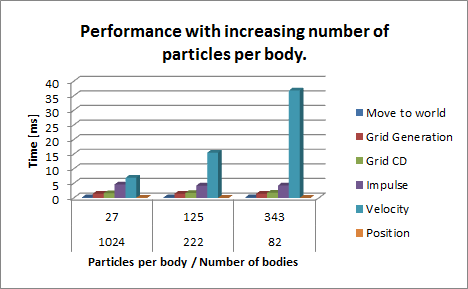
\includegraphics[width = 0.9\textwidth]{particlePerBody.png}
  \caption{Poor scaling for the velocity step with increasing number of particles per body.}
  \label{fig:velScale1}
\end{figure}

\begin{figure}[H]
  \centering
  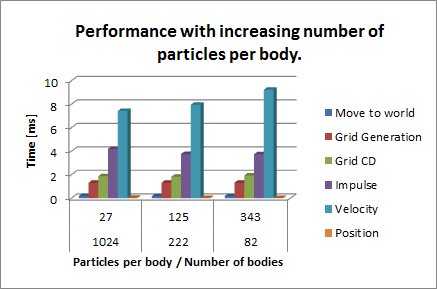
\includegraphics[width = 0.9\textwidth]{particlePerBody2.png}
  \caption{Improved workload gives reasonable scaling for the velocity step with increasing number of particles per body.}
  \label{fig:velScale2}
\end{figure}

The flowchart is updated accordingly to what can be seen in figure~\ref{fig:shaderflow2}.
The calculations performed in the velocity pre-calculation step could just as easily
be implemented into the impulse shader step instead, but has been given a separate shader
step for readability.

\begin{figure}[H]
  \centering
  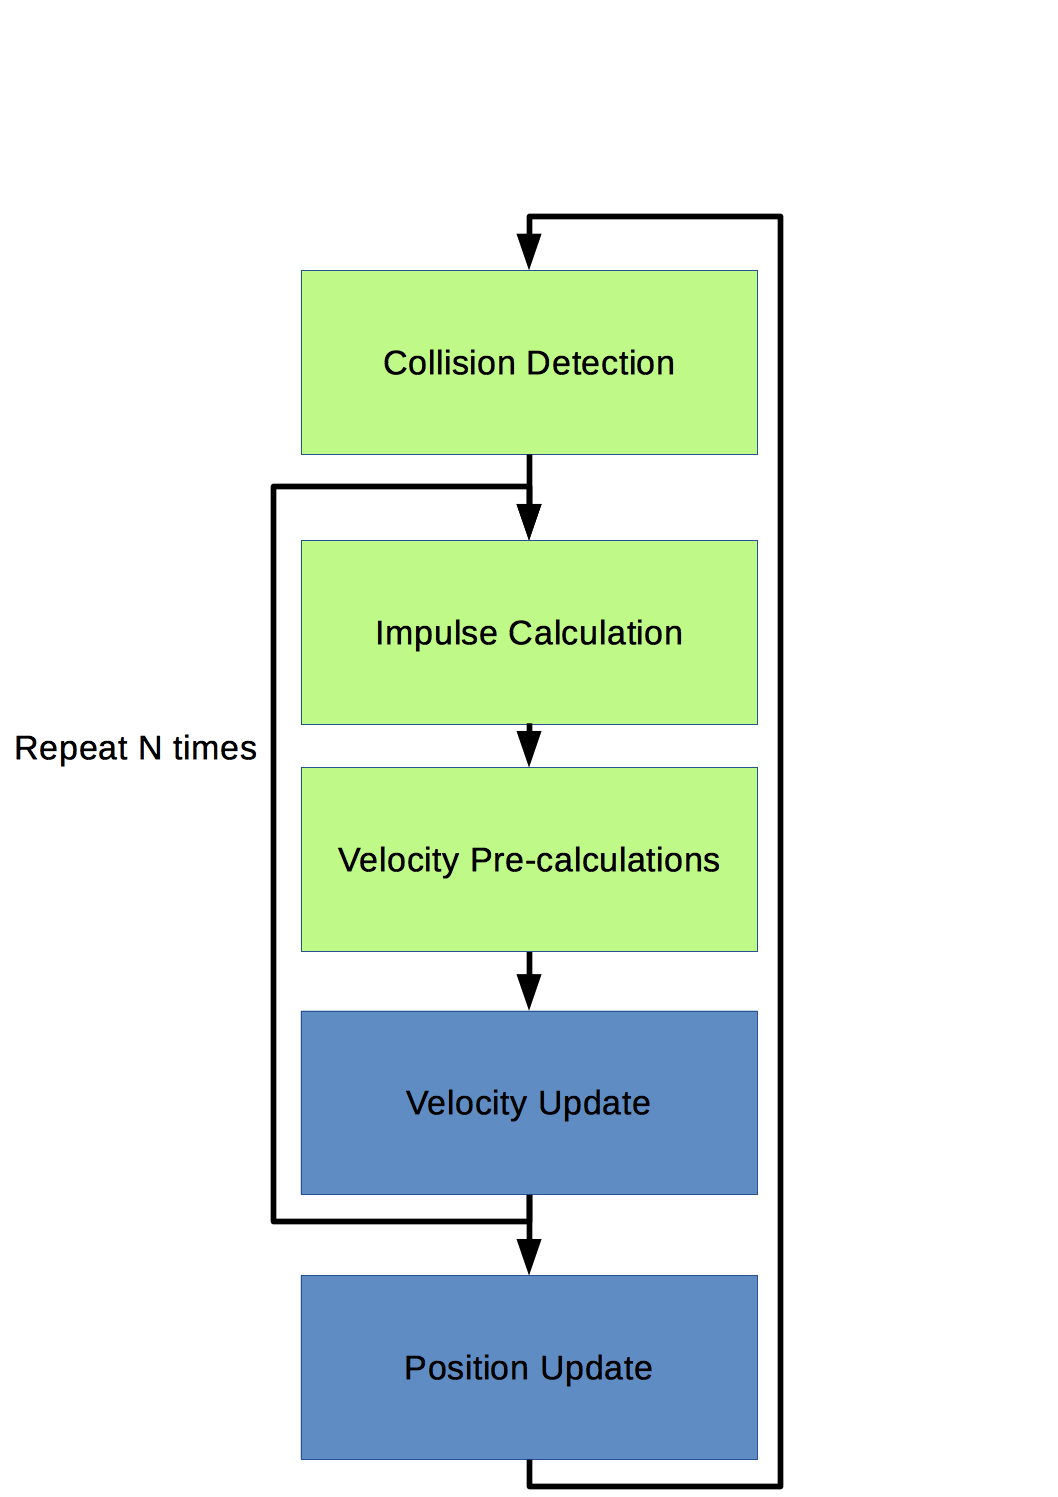
\includegraphics[width = 0.9\textwidth]{shaderflow2.png}
  \caption{Updated flow chart with pre-velocity calculations per particle}
  \label{fig:shaderflow2}
\end{figure}

\subsection{Position Update}
This shader updates the bodies' states through integration as described in the theory chapter.
